\begin{appendices}
	% \chapter{Publicaciones}
	\chapter{miRNAfe: a comprehensive tool for feature extraction in microRNA prediction}
	\label{sec:mirnafe}
	En este trabajo se publicó la herramienta de extracción de características de secuencias tipo tallo-horquilla. Esta publicación corresponde con la primera
	etapa de la metodología desarrollada en al tesis. En este trabajo me encargué de la revisión del estado del arte, del diseño y desarrollo de la biblioteca,
	de la validación de los algoritmos de extracción de características, de la implementación de la interfaz web y de la escritura del manuscrito.
	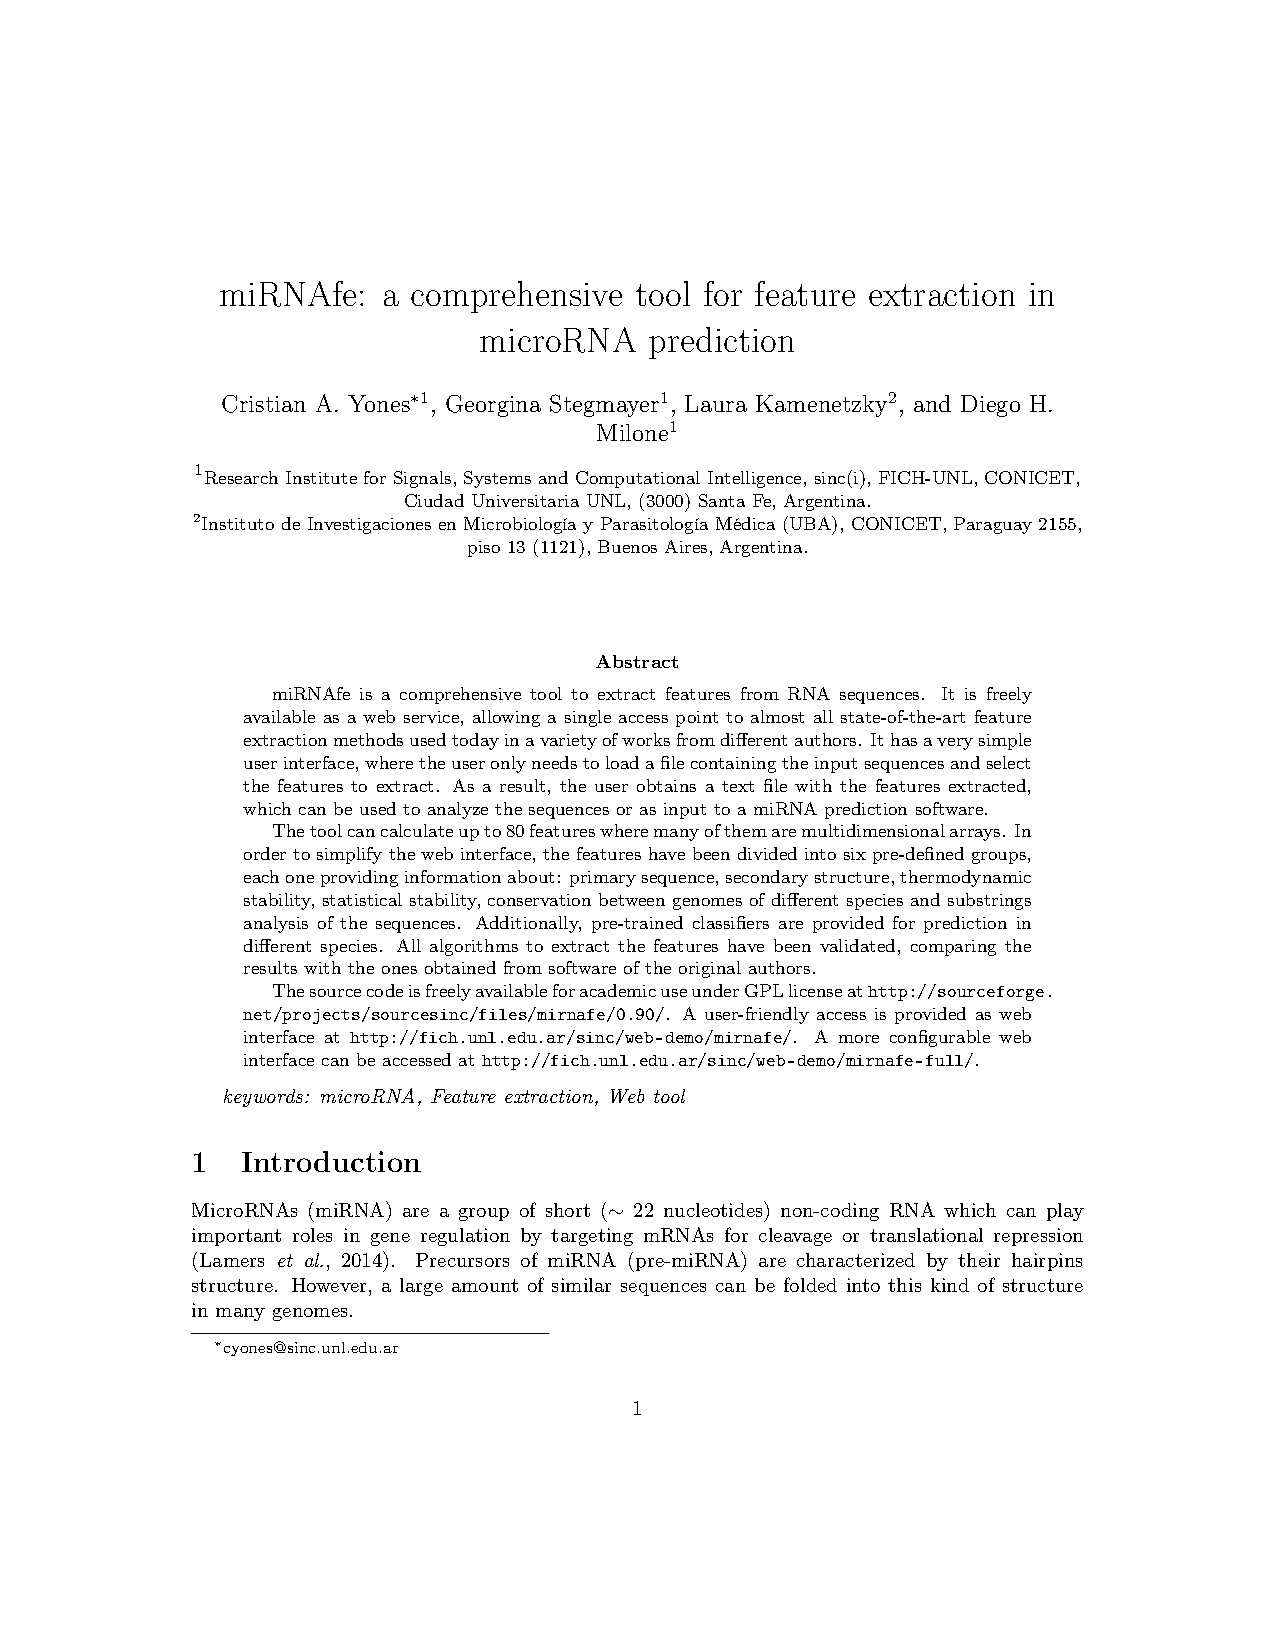
\includepdf[pages=-]{mirnafe/mirnafe.pdf}
	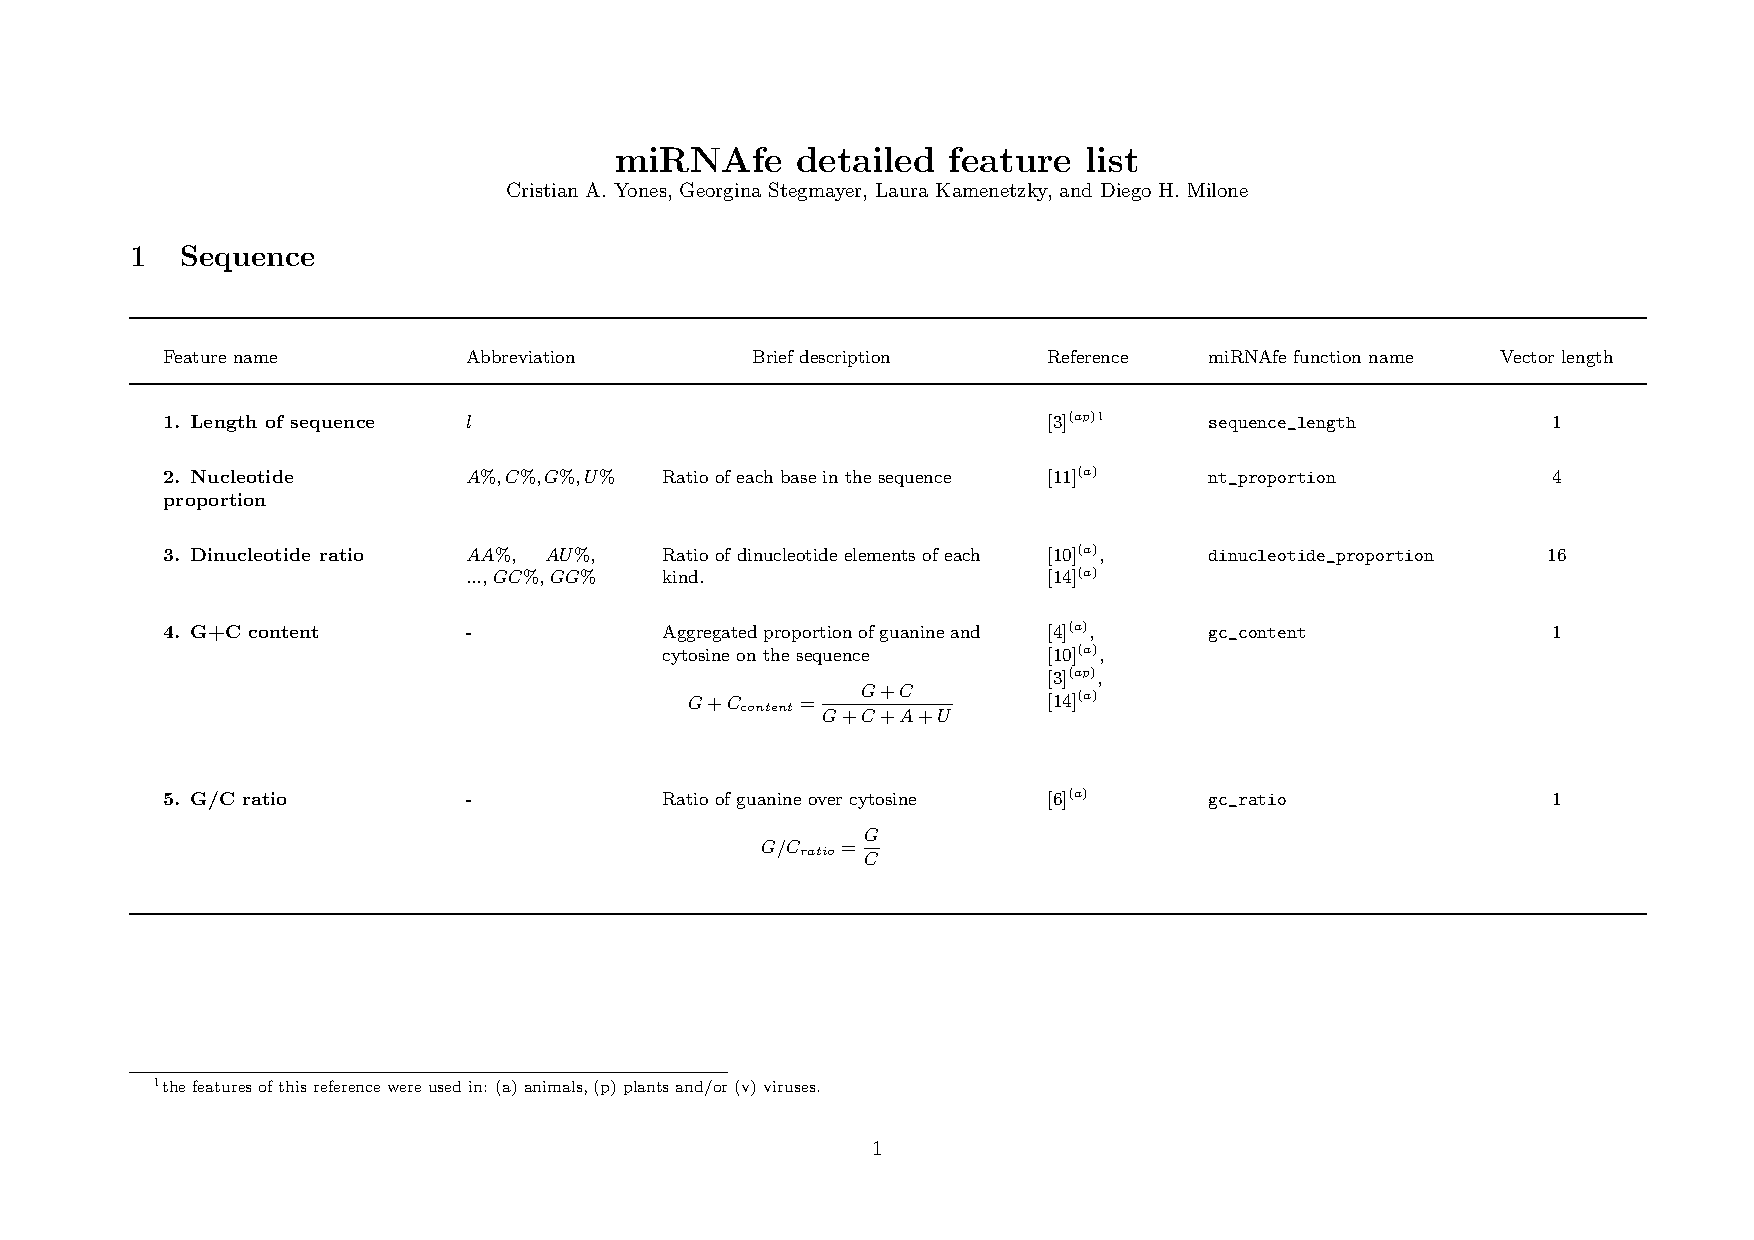
\includepdf[pages=-,angle=90]{mirnafe/supplementary_material.pdf}

	\chapter{Genome-wide pre-miRNA discovery from few labeled examples}
	\label{sec:mirnass}
	En este trabajo se presentó el metodo semi-supervisado de predicción de microRNA en genoma completo. Esta publicación corresponde con la tercera etapa de
	la metodología desarrollada en al tesis. En este trabajo mi contribución fue en el desarrollo de la idea, la ejecución de los experimentos y la redacción
	del manuscrito.
	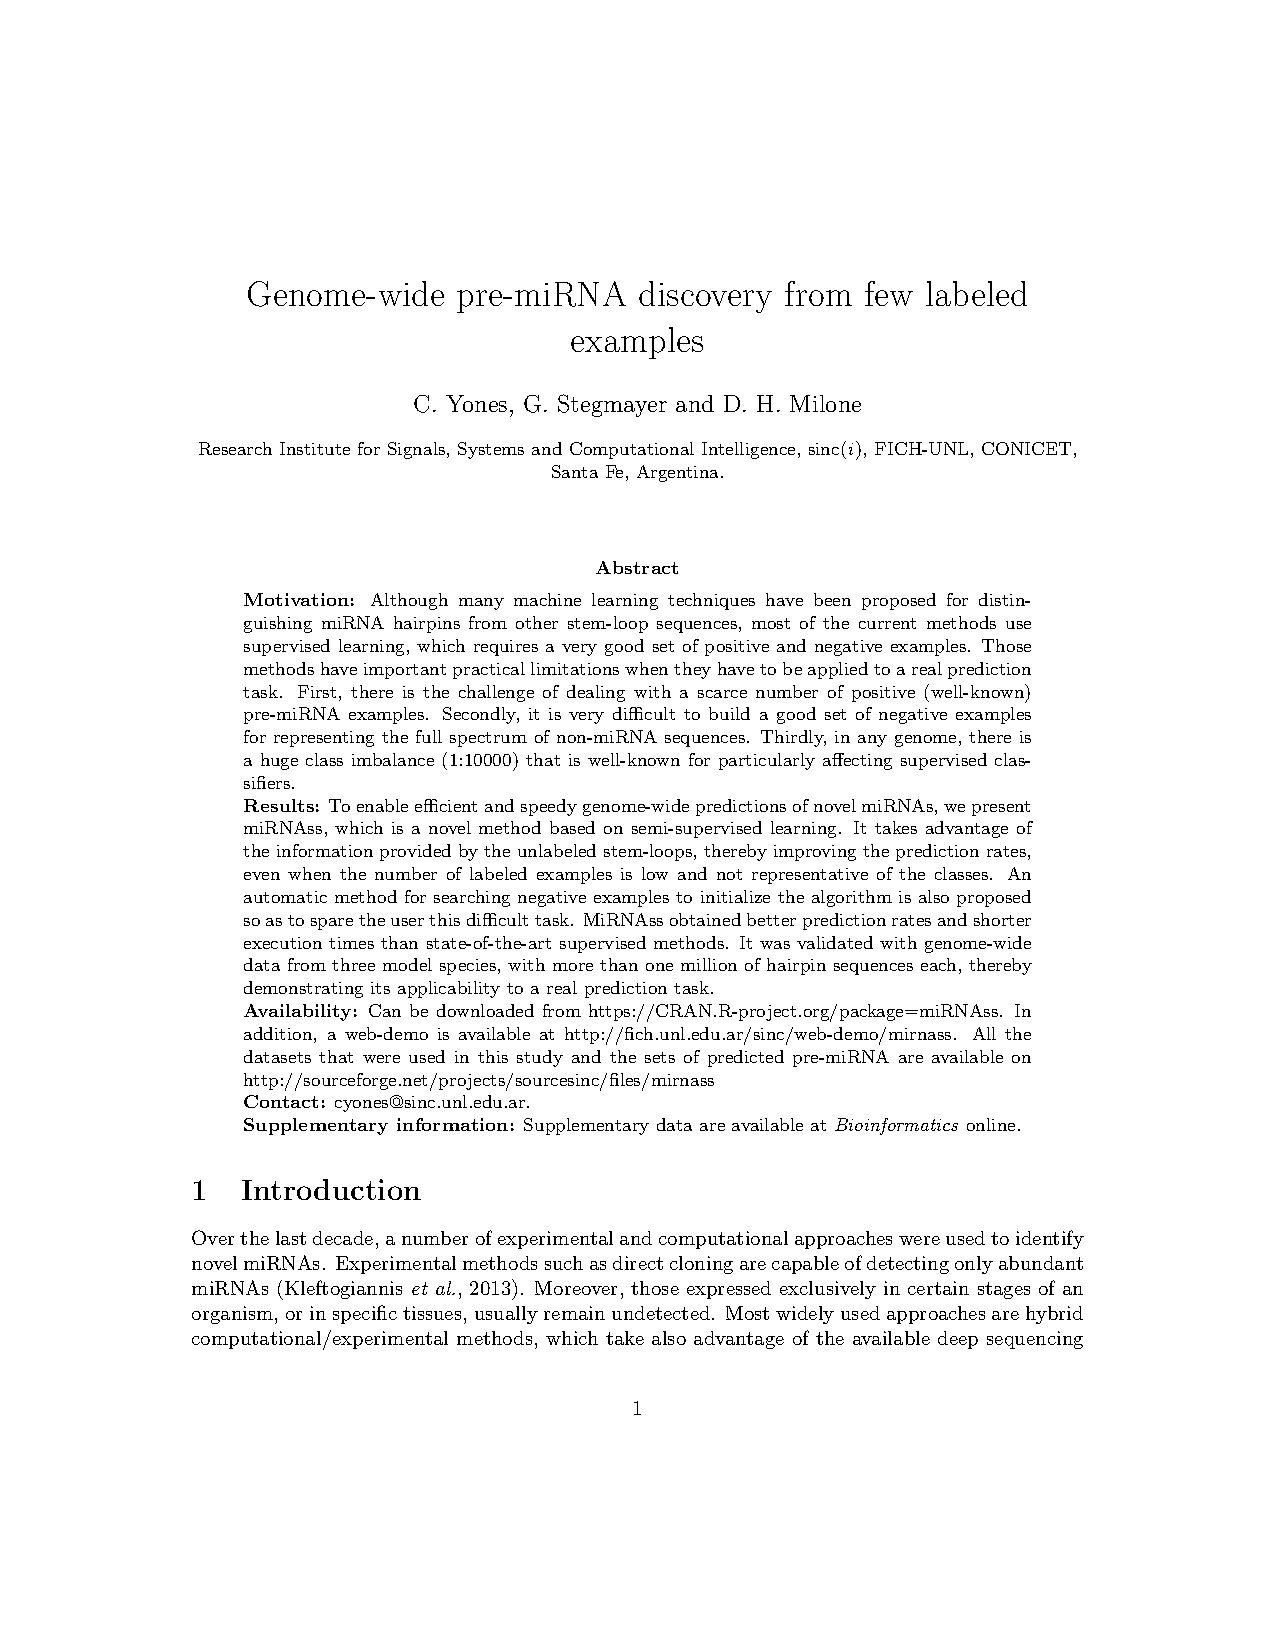
\includepdf[pages=-]{mirnass/mirnass.pdf}
	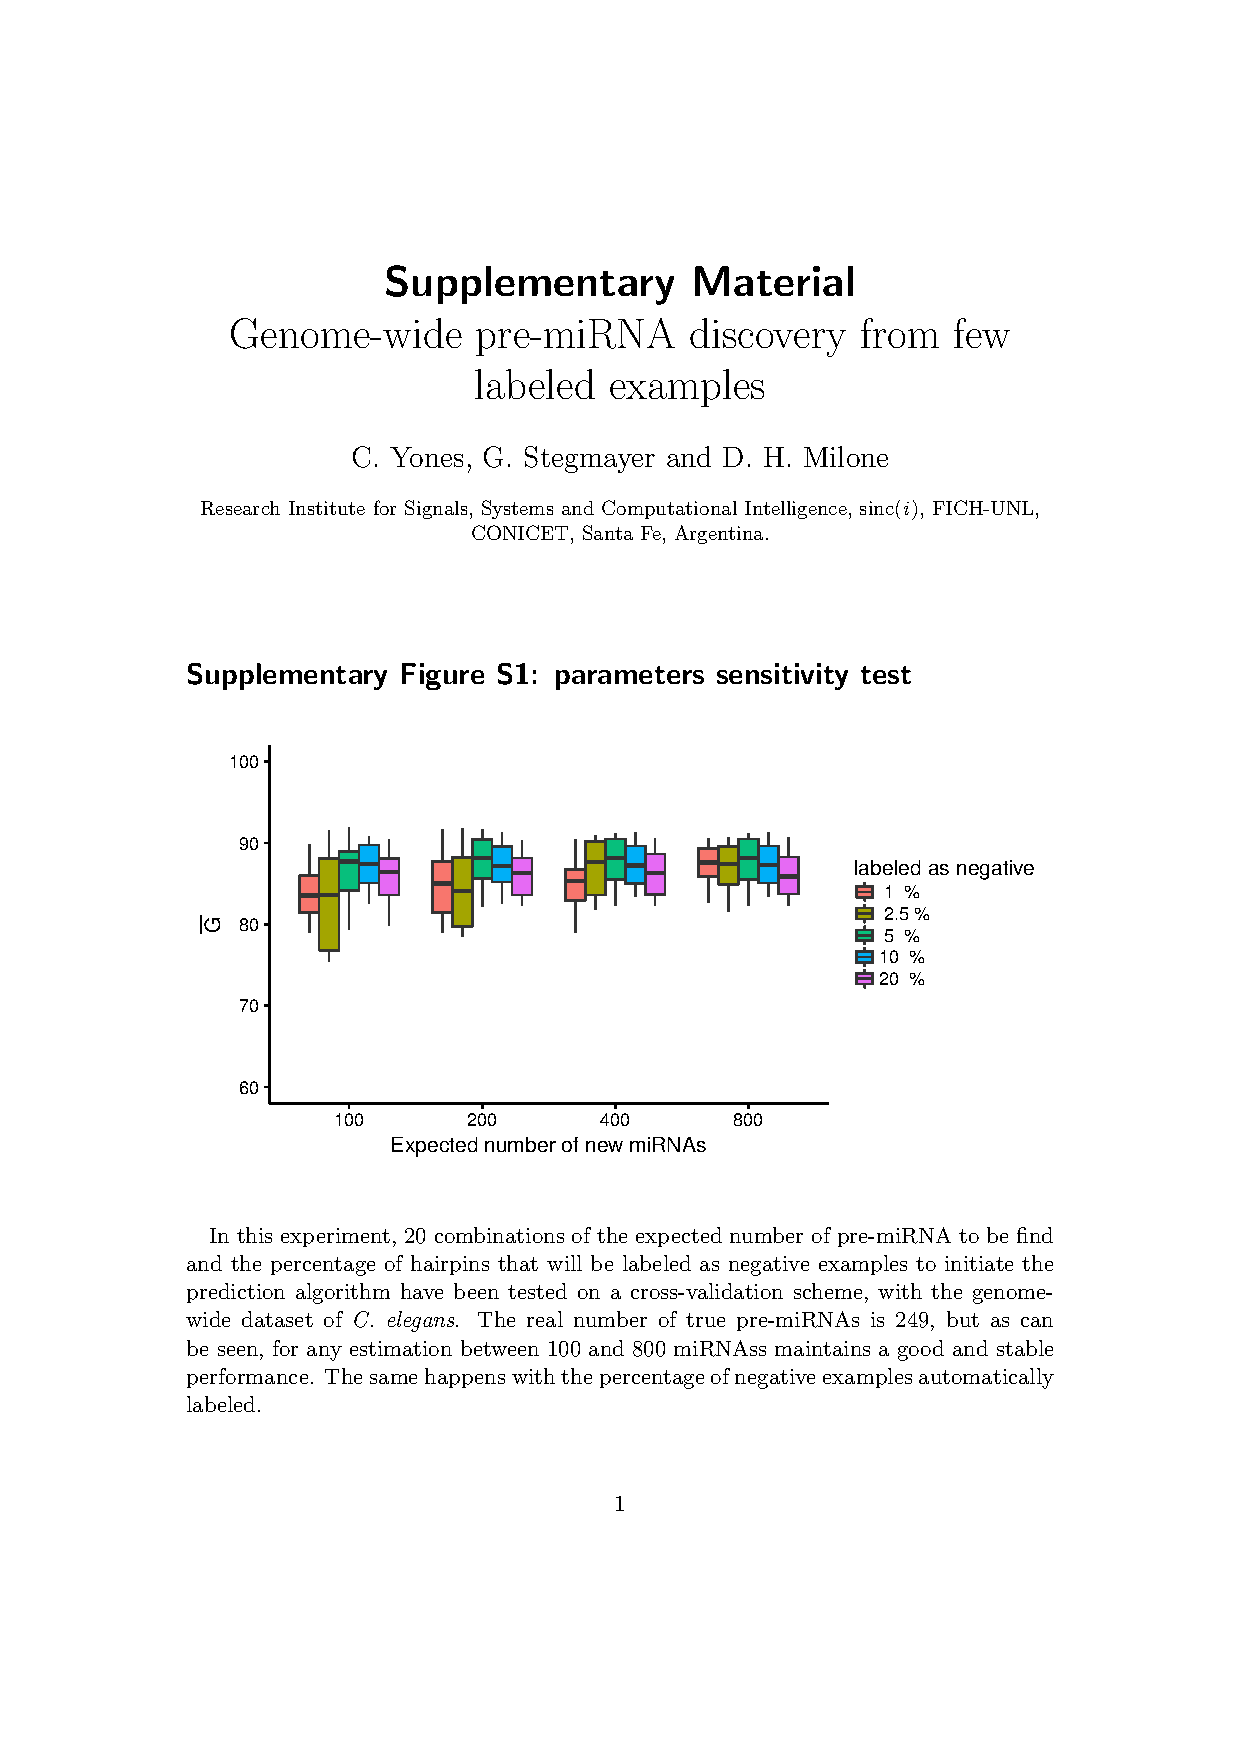
\includepdf[pages=-]{mirnass/supplementary_material.pdf}
\end{appendices}
